\documentclass{standalone}

\usepackage{pgfplots}
\usepackage{pgfplotstable}
\usepackage{filecontents}

\usepackage{tikz}
\usepackage{tikzscale}
\usepackage{tikz-3dplot}
\usepackage{graphicx}

\begin{document}
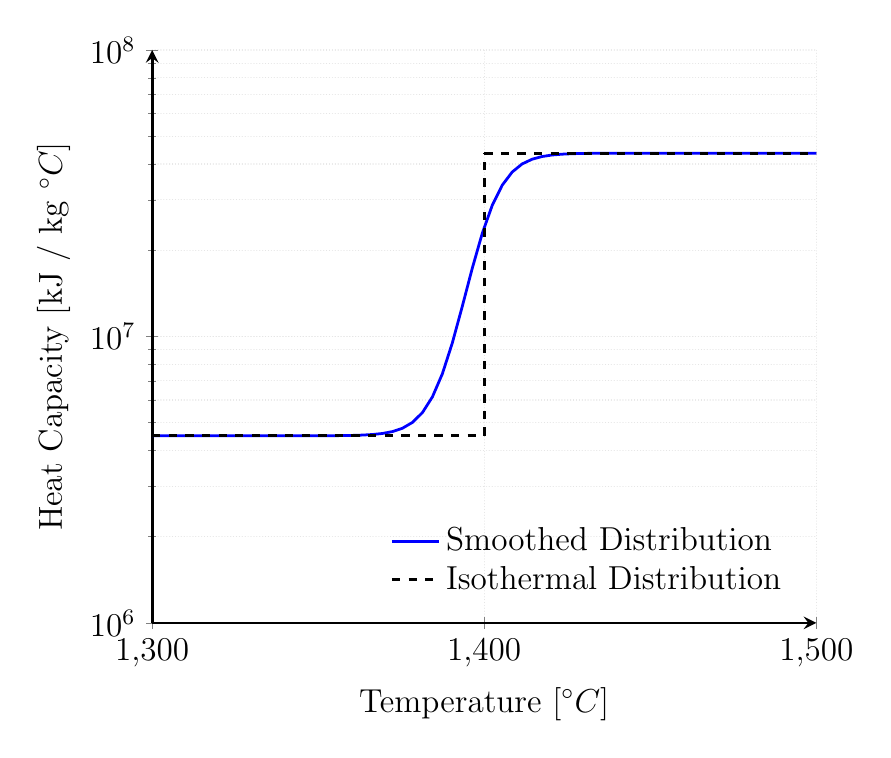
\begin{tikzpicture}

\begin{semilogyaxis}[
        scale only axis, 
	% The height and width argument only apply to the actual axis
        xmin=1300, 
	xmax=1500,
        ymin=1.0e+06, 
	ymax=1.0e+08,
        xlabel={Temperature [$^{\circ}C$]},
        ylabel={Heat Capacity [kJ / kg $^{\circ}C$]},
     	legend pos=south east,
        font=\large,
        mark size=4,
        line width = 1.0,
	legend style={font=\large, mark size=4, fill=none, draw=none},
               legend cell align=left,
    	grid = both,
   	grid style={ dash pattern = on 0.05 off 1, line cap = round, draw=gray!20 },
   	samples=1000,
   	domain=0:3e+03,
%   	restrict y to domain =1.0e+05:3.0e+08,
   	axis lines=left,
   	xtick={1300, 1400, 1500},
    ytick={1e+06, 1e+07, 1.0e+08},
 ]

\addplot[ blue ] plot ( {\x},{ 7500 * 600 + 7500 * 261000 / ( 2.0 * (1450-1400)) * (tanh( (\x - 1400.0) / 10 ) + 1)} );
   \addlegendentry{Smoothed Distribution};
   

 \addplot [black, dashed, no markers] coordinates {(1300, 7500 * 600) (1400, 7500 * 600)};
 \addplot [black, dashed, no markers] coordinates {( 1400, 7500 * 600 ) ( 1400, 7500 * 600 + 7500 * 261000 / 50.0 )};

 \addplot [black, dashed, no markers] coordinates {(1400, 7500 * 600 +  7500.0 * 261000.0 / 50.0 ) (1500, 7500 * 600 +  7500.0 * 261000.0 / 50.0 )};
    \addlegendentry{Isothermal Distribution};
    
\end{semilogyaxis}

\end{tikzpicture}
\end{document}